\subsection[\textit{TorchFrame} (Piotr Winkler)]{\textit{TorchFrame}}
\label{TorchFrame}

  Sztuczne sieci neuronowe stanowią dziedzinę nauki opartą w dużej mierze na
  eksperymentach. Dostarczane przez nie rozwiązania, choć często tak spektakularne,
  są mocno zawoalowane, a droga do celu wiedzie przez kolejne treningi
  i doświadczalny dobór hiperparametrów sieci. Ogromne znaczenie w procesie uczenia
  ma również sposób przetworzenia danych wykorzystywanych do treningów, zarówno
  tych podawanych na wejście sieci, jak i tych otrzymywanych na jej wyjściu.

  Niniejsza praca dotyczy przede wszystkim zastosowania sieci neuronowych w
  procesie przetwarzania obrazów cyfrowych. Wiąże się to z koniecznością przygotowywania
  zbiorów treningowych złożonych z ogromnej ilości danych wizyjnych poddanych
  odpowiedniemu przetworzeniu i filtracji, aby mogły właściwie spełnić swoją rolę
  w czasie treningu sieci.

  Wspomniane zabiegi, jak również konieczność częstego powtarzania treningów,
  wymagają dużych nakładów pracy i czasu, aby mogły przynieść zamierzone efekty.
  W celu ułatwienia całego procesu przygotowany został framework \textit{TorchFrame}
  stanowiący bazę pod eksperymenty podejmowane w ramach tej pracy i opisane w
  dalszych jej rozdziałach.

  Sam framework umożliwia użytkownikom przeprowadzanie treningów sieci neuronowych,
  udostępniając wachlarz modyfikowalnych hiperparametrów oraz zestaw filtrów i metod
  przeznaczonych do obróbki danych treningowych. Właściwie użyty \textit{TorchFrame} kontroluje
  przepływ danych uczących od początku do końca ograniczając konieczność ingerencji ze
  strony użytkownika do minimum, jednocześnie nie ograniczając przy tym potencjału
  eksperymentalnego sztucznych sieci neuronowych.

  W ramach frameworka udostępniony został również prosty interfejs testowy
  umożliwiający ocenę efektów uzyskanych w procesie uczenia.

  Niniejszy rozdział zostanie poświęcony analizie architektury \textit{TorchFrame'a} oraz
  opisowi sposobu jego działania.

  \subsubsection{\textit{PyTorch}}

    U podstaw \textit{TorchFrame'a} leżą mechanizmy innego frameworka, napisanego w języku Python i
    przeznaczonego do uczenia maszynowego o nazwie \textit{PyTorch}. Jest to otwartoźródłowa
    biblioteka programistyczna stworzona przez oddział sztucznej inteligencji firmy
    Facebook. W jednym z artykułów \cite{pytorch} opublikowanych w ramach konferencji NIPS 2017
    grupa badaczy opisuje ją następująco:

    \begin{quote}
      'PyTorch - biblioteka zaprojektowana w celu umożliwienia szybkiego badania
      modeli uczenia maszynowego. Bazuje na kilku projektach, głównie Lua Torch,
      Chainer i HIPS Autograd, oraz dostarcza wysoko wydajnościowe środowisko z
      łatwym dostępem do automatycznego różnicowania modeli wykonywanych na różnych
      urządzeniach (CPU i GPU). Aby uczynić prototypowanie łatwiejszym, PyTorch
      nie podąża za podejściem symbolicznym używanym w wielu innych frameworkach
      do uczenia głębokiego, ale skupia się na różnicowaniu czysto imperatywnych
      programów, skupiając się na rozszerzalności i małym narzucie.' (...)

      'PyTorch, podobnie jak większość innych bibliotek do uczenia głębokiego obsługuje
      automatyczne różnicowanie funkcji skalarnych w trybie wstecznym, czyli jedną z najważniejszych form
      automatycznego różnicowania dla aplikacji uczenia głębokiego, które zwykle
      różnicują skalarną funkcję celu.'
    \end{quote}

    \textit{TorchFrame} wykorzystuje zdefiniowane w ramach \textit{PyTorch'a} mechanizmy budowania sieci neuronowych
    korzystając z predefiniowanych metod opisu warstw sieci. Wykorzystuje ponadto
    zdefiniowane odgórnie hiperparametry, takie jak funkcje kosztu. Sam rdzeń \textit{TorchFrame'a}
    bazuje na przytoczonym mechanizmie różnicowania, umożliwiając przeprowadzanie treningów
    na CPU oraz GPU.

  \subsubsection{Architektura \textit{TorchFrame}}

    \textit{TorchFrame} podzielony został na bloki funkcjonalne, które powiązane ze sobą
    umożliwiają kontrolowany przepływ danych w procesie uczenia, a jednocześnie
    zapewniają elastyczność przy wprowadzaniu rozmaitych modyfikacji. Schemat funkcjonalny
    całego systemu przedstawiony został na Rysunku \ref{fig:torchframetrain}.

      \begin{figure}[h!]
        \centering
        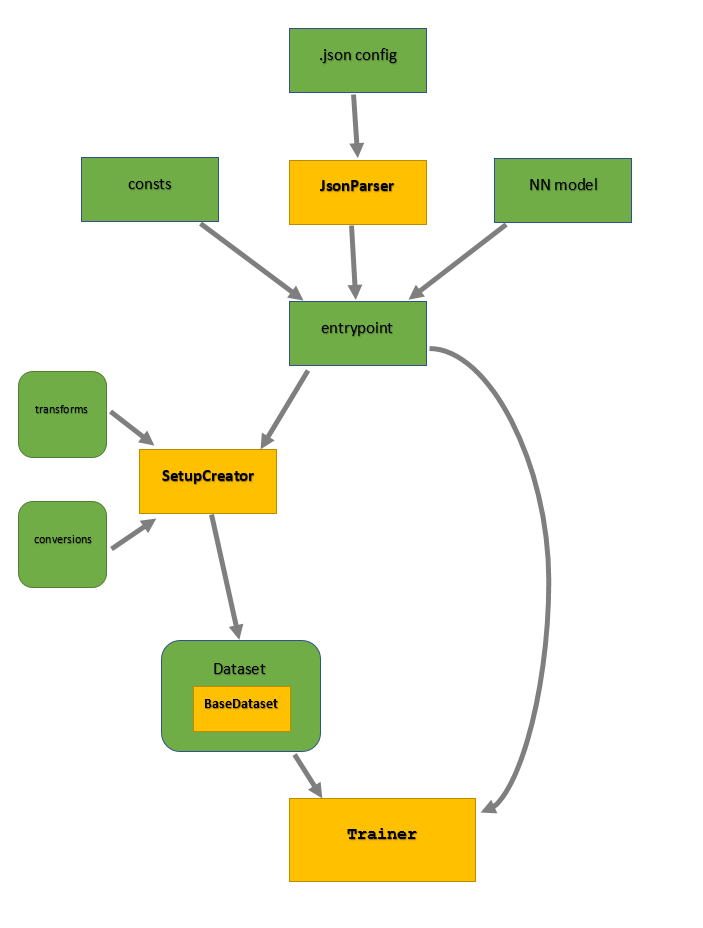
\includegraphics[width=5.5in]{torchframetrain}
        \caption[Architektura \textit{TorchFrame} - źródło: Rysunek własny]{Architektura \textit{TorchFrame}}
        \label{fig:torchframetrain}
      \end{figure}

    Przepływ danych przez framework rozpoczyna się w obrębie trzech plików konfiguracyjnych,
    oznaczonych na przytoczonym schemacie odpowiednio jako: \textit{consts}, \textit{.json config}
    oraz \textit{NN model}.

    W pliku \textit{consts} użytkownik \textit{TorchFrame} definiuje zmienne środowiskowe, takie, jak
    ścieżki do plików kluczowych w procesie uczenia. Konieczne jest jedynie wskazanie
    położenia pliku konfiguracyjnego w formacie \textit{JSON}. Pozostałe parametry są opcjonalne
    i mogą służyć do wskazania miejsca zapisu gotowego modelu sieci na dysku czy miejsca
    przechowywania danych treningowych, które zostaną następnie przetworzone i przekazane
    na wejście sieci w procesie uczenia.

    \textit{NN model} to skrypt języka Python, w którym użytkownik definiuje strukturę sieci
    neuronowej zgodnie z paradygmatem frameworka \textit{PyTorch} przytoczonego w poprzednim
    rozdziale. Struktura \textit{TorchFrame} narzuca na użytkownika konieczność zdefiniowania
    metody \textit{forward}, która określa sposób obliczania wartości wyjściowych sieci na podstawie danych
    wejściowych między innymi poprzez określenie funkcji aktywacji poszczególnych warstw
    sztucznych neuronów.

    Najważniejszym punktem zestawu konfiguracyjnego jest wspomniany już plik \textit{JSON}.
    Udostępnia on szerokie możliwości manipulowania zarówno hiperparametrami sieci
    neuronowej, jak i szeregiem przekształceń możliwych do zaimplementowania
    na danych treningowych i testowych. Architektura \textit{TorchFrame} zapewnia odpowiednie
    rozpropagowanie zgromadzonych tutaj danych w ramach procesu uczenia oraz podczas
    testów. Dokładna struktura tego pliku zostanie opisana w następnym rozdziale.

    \textit{JsonParser} jest klasą odpowiedzialną za odczytanie danych z pliku konfiguracyjnego,
    w formie słownika języka Python, oraz przekazanie ich w dalszą drogę w obrębie \textit{TorchFrame}.

    Centralnym punktem całej zaprezentowanej architektury jest \textit{entrypoint}. Stanowi on
    punkt wejścia dla aplikacji użytkownika. Jego uruchomienie powoduje
    agregację danych ze wspomnianych już plików konfiguracyjnych, pogrupowanie ich
    oraz rozpropagowanie do dalszych komponentów odpowiedzialnych za przetwarzanie
    danych treningowych oraz przeprowadzanie samego treningu sieci neuronowej.

    Część danych przekazywanych przez \textit{entrypoint} trafia do \textit{SetupCreator'a}. Komponent
    ten odpowiada za skomponowanie listy konwersji wymienionych w pliku
    konfiguracyjnym. Konwersje te zostaną następnie zaimplementowane na danych treningowych
    na etapie tworzenia zbioru uczącego. Źródłem danych do którego odwołuje się
    \textit{SetupCreator} są skrypty \textit{transforms} oraz \textit{conversions}. Zawierają one gotową bazę
    przekształceń przeznaczonych do pracy na obrazach cyfrowych, a także metody
    formatowania danych do struktury \textit{tensorów} (przypominających macierze z biblioteki \textit{numpy}
    języka Python) wykorzystywanych przez bibliotekę \textit{PyTorch} między innymi w mechanizmach
    automatycznego różnicowania modeli sieci neuronowych. Choć gotowa baza oferuje
    liczne przekształcenia, intuicyjna formuła pozwala użytkownikom w łatwy sposób definiować
    własne metody konwersji i implementować je zarówno na obrazach, jak i dowolnym innym
    rodzaju danych treningowych.

    Tak skomponowany zestaw przekształceń wykorzystywany jest przy konstruowaniu zbioru
    uczącego w komponencie \textit{Dataset}. Jego uniwersalny szkielet o nazwie \textit{BaseDataset}
    odpowiada za sprawny przepływ danych w ramach \textit{TorchFrame} zapewniając łatwy dostęp
    do zbioru implementowanych konwersji oraz umożliwiając ich zastosowanie poprzez dedykowane
    do tego metody. Posiada również funkcjonalność odczytu danych ze wskazanej przez
    użytkownika ścieżki w pliku \textit{consts}, a także zdolność przetwarzanie ich na bieżąco, co pozwala
    zaoszczędzić pamięć w przypadku pracy na dużych zbiorach danych. W ramach tworzenia
    frameworka \textit{TorchFrame} udostępnione zostały różne implementacje komponentu \textit{Dataset} opierające się o
    \textit{BaseDataset}. Ponownie jednak elastyczna struktura umożliwia użytkownikom
    skomponowanie własnych implementacji dostosowanych do indywidualnych potrzeb.

    Ostatecznym elementem ścieżki treningowej, w którym skupiają się wszystkie
    zgromadzone dotąd dane jest komponent \textit{Trainer}. Opiera się on o mechanizmy
    frameworka \textit{PyTorch} w celu obliczania rezultatów pracy sieci, a także wyznaczanie
    kierunku uczenia w ramach funkcji celu i wstęczną propagację modyfikującą wagi
    sieci w czasie treningu. \textit{Trainer} udostępnia na bieżąco dane pozwalające
    określić skuteczność uczenia sieci takie jak aktualny błąd sieci, ilość
    przetworzonych danych, czy numer epoki treningowej, w której aktualnie znajduje
    się model. W trakcie całego procesu możliwe jest również zapisywanie rezultatów
    w celu ich ponownego wykorzystania lub oceny.

  \subsubsection{Konfiguracja w \textit{TorchFrame}}

    Kluczem do właściwego przeprowadzenia treningu sztucznej sieci neuronowej
    jest odpowiedni dobór hiperparametrów. Ich modyfikacja w znaczący sposób
    wpływa na otrzymywane rezultaty przez co istotne jest, aby w ramach
    kolejnych eksperymentów można było w łatwy sposób dostosowywać je do potrzeb.
    Framework \textit{TorchFrame} udostępnia pojedynczy interfejs użytkownika w postaci
    pliku konfiguracyjnego \textit{JSON} skupiającego wszystkie najistotniejsze
    elementy w jednym miejscu i pozwalającego zachować przejrzystość stosowanej
    konfiguracji. W poniższym rozdziale opisane zostaną dostępne parametry wraz
    z wartościami, jakie mogą przyjmować.

    \begin{enumerate}
    \item \textbf{\textit{Net model}} - ten parametr przyjmuje nazwę klasy, w której użytkownik
    zdefiniował strukturę sieci neuronowej na etapie inicjalizacji wraz z metodą
    \textit{forward} definiującą sposób przepływu danych w ramach inferencji modelu.
    \item \textbf{\textit{Criterion}} - parametr ten pozwala zdefiniować funkcję kosztu
    używaną w procesie uczenia. W czasie treningu sieci neuronowych dąży się
    najczęściej do minimalizacji błędu określanego na bazie porównania rezultatów
    pracy sieci ze spodziewanym efektem. Zdefiniowana na tej podstawie funkcji błędu
    określana jest jako funkcja celu, a proces uczenia sieci sprowadza się do zdefiniowania
    zestawu wag, dla których jej wartość jest możliwie najmniejsza. Zagadnienie
    to opisane zostało w książce \textit{Deep Learning} \cite{deeplearn} z 2016 roku:

    \begin{quote}
      'Funckja, którą chcemy minimalizować, lub maksymalizować nazywana jest funkcją celu lub kryterium.
      W przypadku minimalizacji możemy również nazywać ją funkcją kosztu, funkcją straty, lub funkcją błędu.'
    \end{quote}

    Na funkcji kosztu spoczywa bardzo ważne zadanie. Musi ona wiernie destylować wszystkie
    aspekty modelu w jedną liczbę, w taki sposób, aby ulepszenia tej liczby były
    oznaką poprawy całego modelu. \cite{neuralsmithing}

    \begin{quote}
      'Funkcja kosztu redukuje wszystkie dobre i złe aspekty potencjalnie złożonego
      systemu do pojedynczej liczby, wartości skalarnej, która umożliwia
      klasyfikację i porównanie możliwych rozwiązań.'
    \end{quote}

    Dobór odpowiedniej funkcji kosztu może stanowić spore wyzwanie, ponieważ funkcja
    ta musi uchwycić właściwości danego problemu i być motywowana założeniami
    istotnymi z punktu widzenia realizowanego projektu. \cite{neuralsmithing}

    \begin{quote}
      '(...) Dlatego ważne jest, aby funkcja wiernie reprezentowała nasze cele projektowe.
      Jeśli wybierzemy słabą funkcję błędu i uzyskamy niezadowalające wyniki, to
      wina za złe określenie celu poszukiwań spoczywa na nas.'
    \end{quote}

    Opisy rozmaitych funkcji kosztu dostępnych w \textit{TorchFrame}, zaczerpniętych z biblioteki \textit{PyTorch},
    zamieszczone zostały w tabeli \ref{tab:cost_functions}.
 \begin{small}
    \begin{longtable}{ |m{2cm}|m{11cm}| }
      \caption{Funkcje kosztu w \textit{TorchFrame}}
      \label{tab:cost_functions}
      \endfirsthead
      \endhead
     \hline
       \textbf{Funkcja kosztu} & \textbf{Opis} \\

     \hline
       \textbf{L1Loss} &

       Funkcja kosztu mierząca średni błąd bezwzględny pomiędzy
       odpowiadającymi sobie elementami ze zbioru wejściowego i docelowego.
       Można ją opisać za pomocą następującego wzoru:

       \[l(x,y) = L = \{l_1,...,l_N\}^T, l_n = |x_n - y_n|,\]

       gdzie \textit{N} jest rozmiarem pojedynczego pakietu danych, a \textit{x} i
       \textit{y} to tensory o arbitralnym kształcie, z których każdy posiada
       \textit{n} elementów.

       Parametry:
       \begin{itemize}
       \item reduction - parametr ten może przyjmować trzy wartości \textit{none},
       \textit{mean} oraz \textit{sum}. Pierwsza opcja spowoduje, że wartość funkcji
       celu zostanie wyznaczona zgodnie z podanym powyżej wzorem. Wartość \textit{mean}
       spowoduje wyznaczenie średniej wartości elementów wyjściowych. \textit{Sum}
       oznacza natomiast, że wyznaczona zostanie ich suma.
       \end{itemize} \\

     \hline
       \textbf{MSELoss} &

       Funkcja kosztu mierząca średni błąd kwadratowy pomiędzy każdym elementem
       wejściowym \textit{x} i celem \textit{y}. Opisuje ją poniższy wzór:

       \[l(x,y) = L = \{l_1,...,l_N\}^T, l_n = (x_n - y_n)^2,\]

       gdzie \textit{N} jest rozmiarem pojedynczego pakietu danych, a \textit{x} i
       \textit{y} to tensory o arbitralnym kształcie, z których każdy posiada
       \textit{n} elementów.

       Parametry:
       \begin{itemize}
       \item reduction - czytaj \textit{reduction} dla funkcji \textit{L1Loss}.
       \end{itemize} \\

     \hline
       \textbf{KLDivLoss} &

       Funkcja kosztu nazywana rozbieżnością Kullback'a - Leibler'a. Jest użyteczną
       miarą dla rozkładów ciągłych i często jest przydatna podczas wykonywania
       bezpośredniej regresji w przestrzeni (dyskretnie próbkowanych) ciągłych
       rozkładów wyjściowych.

       Kryterium to wymaga, aby rozmiary tensorów wejściowych i wyjściowych były
       identyczne.

       Wzór matematyczny opisujący rozbieżność KL przedstawiony został poniżej:

       \[l(x,y) = L = \{l_1,...,l_N\}, l_n = y_n \cdot (\log_{}y_n - x_n),\]

       gdzie indeks \textit{N} obejmuje wszystkie wymiary wejściowe, a \textit{L}
       ma ten sam kształt, co wejście.

       Parametry:
       \begin{itemize}
       \item reduction - poza wartościami opisanymi dla funkcji \textit{L1Loss}
       może przyjmować również parametr \textit{batchmean}. Wymusza on sumowanie
       wartości wyjściowych, a następnie podział sumy przez rozmiar pakietu danych.
       \end{itemize} \\

     \hline
       \textbf{BCELoss} &

       Kryterium wyznaczające wartość Binarnej Entropii Krzyżowej pomiędzy wyjściem
       sieci, a spodziewanymi rezultatami jej pracy.

       Opisuje to poniższy wzór:

       \[l(x,y) = L = \{l_1,...,l_N\}^T, l_n = -w_n[y_n \cdot \log_{}x_n + (1 - y_n) \cdot \log_{}(1 - x_n)],\]
       \[w_n = waga[n],\]

       gdzie \textit{N} jest rozmiarem pakietu danych.

       Parametry:
       \begin{itemize}
       \item \textit{weight} - manualna wartość wagi przeskalowującej funkcję kosztu
       każdego elementu w pakiecie danych.
       \item \textit{reduction} - czytaj \textit{reduction} dla funkcji \textit{L1Loss}.
       \end{itemize} \\

     \hline
     \textbf{SmoothL1-
     Loss} &

       Kryterium przyjmujące postać funkcji \textit{MSE} w przypadku, gdy wartość
       błędu bezwzględnego spada poniżej 1 oraz funkcji \textit{L1} w przeciwnym
       wypadku. Funkcja ta jest mniej czuła na wartości odstające niż
       \textit{MSELoss}, a w niektórych przypadkach zapobiega zjawisku
       eksplodującego gradientu. Znana jest również jako funkcja kosztu \textit{Huber'a}.

       Wzór opisujący:

       \[loss(x,y) = \frac{1}{n}\sum_{i}^{}z_i,\]

       gdzie $z_i$ zdefiniowane jest następująco:

       \[
       y = \left\{ \begin{array}{ll}
       0.5 \cdot (x_i - y_i)^2 & \textrm{gdy $|x_i - y_i| < 1$}\\
       |x_i - y_i| - 0.5 & \textrm{gdy $|x_i - y_i| \ge 1$}
       \end{array} \right.
       \]

       Parametry:
       \begin{itemize}
       \item reduction - czytaj \textit{reduction} dla funkcji \textit{L1Loss}.
       \end{itemize} \\

     \hline
    \end{longtable}
 \end{small}

    \item \textbf{\textit{Optimizer}} - pozwala wybrać rodzaj optymalizatora używanego w procesie
    uczenia sieci neuronowej. Jest to algorytm odpowiedzialny za aktualizowanie
    wag modelu. Korzysta on z wartości funkcji kosztu, jak z drogowskazu
    wskazującego kierunek prowadzący do osiągnięcia globalnego minimum w
    procesie minimalizacji, jakim jest trening sieci.

    Zadanie zlokalizowania globalnego minimum nie jest zadaniem trywialnym.
    Optymalizacja sieci neuronowych jest optymalizacją niewypukłą. Oznacza to, że
    funkcja celu posiada wiele optimów, z czego tylko jedno jest poszukiwanym
    optimum globalnym. Przykładowa płaszczyzna funkcji celu przedstawiona
    została na Rysunku \ref{fig:plaszczyzna_optymalizacji}.

    \begin{figure}[H]
      \centering
      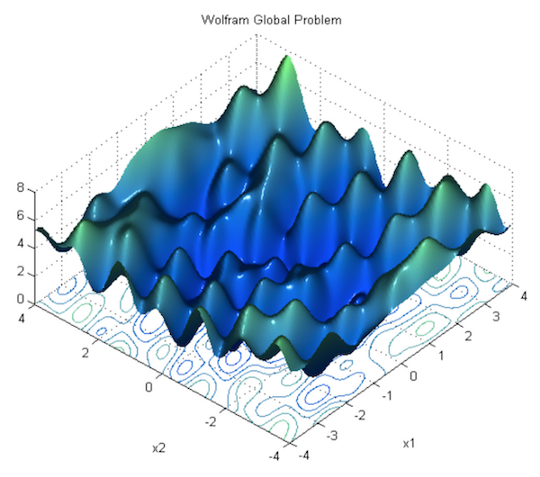
\includegraphics[width=4in]{plaszczyzna_optymalizacji}
      % \caption[Przykładowa płaszczyzna funkcji celu - źródło: \url{https://towardsdatascience.com/neural-network-optimization-7ca72d4db3e0}]{Przykładowa płaszczyzna funkcji celu}
      \caption[Przykładowa płaszczyzna funkcji celu - źródło: \url{https://towardsdatascience.com}]{Przykładowa płaszczyzna funkcji celu}
      \label{fig:plaszczyzna_optymalizacji}
    \end{figure}

    Można powiedzieć, że argumentami funkcji celu są wagi modelu sieci neuronowej.
    Każde kolejne połączenie w sieci posiadające własną wagę zwiększa wymiar
    płaszczyzny poszukiwań. Oznacza to, że dla modelu opisanego trzema wagami
    obszarem poszukiwań będzie płaszczyzna trójwymiarowa. Zazwyczaj modele sieci
    są jednak dużo większe. I tak dla modelu, na który składa się przykładowo sto
    wag poszukiwania optimum są w rzeczywistości prowadzone na hiperpłaszczyźnie
    posiadającej sto wymiarów.

    Najbardziej podstawowym algorytmem optymalizacji leżącym u podstaw innych
    metod jest tak zwany spadek gradientu. Najlepiej opisuje go programistyczna
    formuła aktualizacji wag sieci:

    \[\Theta = \Theta - \eta \cdot \nabla J(\Theta),\]

    gdzie $\eta$ jest długością kroku treningowego, a $\nabla J(\Theta)$ oznacza
    gradient funkcji kosztu zależnej od wag sieci $\Theta$. Warto zauważyć, że
    wartość gradientu wskazuje na płaszczyźnie funkcji celu położenie maksimum,
    dlatego w procesie minimalizacji musimy kierować się w przeciwną stronę i odejmować
    gradient od wag modelu.

    Sam gradient wyznaczany jest z wykorzystaniem bardzo popularnego obecnie
    algorytmu nazywanego propagacją wsteczną. Jego ogólna idea jest stosunkowo
    prosta. Rezultaty pracy sieci ewaluowane są względem pożądanych wyników w
    ramach opisanej w poprzednim punkcie funkcji celu. Jeśli wyniki oceny nie są
    zadowalające wagi sieci są modyfikowane, a cała operacja powtarzana jest aż
    do momentu zakończenia treningu.

    Raul Rojas w swojej książce \cite{systematic_introduction} z 1996 roku tak
    opisuje etapy tego algorytmu:

    \begin{quote}
      'Rozważmy sieć neuronową z pojedynczym wejściem rzeczywistym $x$ i funkcją
      sieci $F$. Pochodna $F(x)$ jest obliczana w dwóch fazach:

      Przekazywanie: wejście $x$ jest podawane do sieci. Funkcje aktywacji i ich pochodne są oceniane w każdym węźle (neuronie) sieci. Pochodne są przechowywane.

      Propagacja wsteczna: stała 1 jest podawana do jednostki wyjściowej i sieć biegnie wstecz. Informacje przychodzące do węzła są dodawane, a wynik jest mnożony przez wartość zmagazynowaną w lewej części jednostki. Rezultat jest transmitowany na lewo od jednostki. Wynik zgromadzony w jednostce wejściowej stanowi pochodną funkcji sieci względem $x$.'
    \end{quote}

    Sam algorytm wstecznej propagacji działa poprawnie również dla sieci posiadających
    więcej niż jedną jednostkę wejściową, w których zaangażowanych jest więcej
    niezależnych zmiennych. Idea jego działania pozostaje wówczas ta sama.

    Wynika z tego, że algorytm wstecznej propagacji, a co za tym idzie czerpiący z
    niego w czystej postaci spadek gradientu, cechują się dużą stałością i
    przewidywalnością działania. W wielu przypadkach jest to pożądana cecha, jednak
    zwiększająca się ilość parametrów sieci może powodować pojawianie się trudności
    wymagających od algorytmów optymalizacji większej elastyczności w podejmowaniu działań.

    Do trudności takich zaliczyć można między innymi dobór odpowiedniej długości
    kroku treningowego tak, aby znaleźć złoty środek między szybkością wyznaczenia
    rozwiązania, a jego dokładnością. Dodatkowo w przypadku wspomnianych algorytmów
    wszystkie parametry sieci modyfikowane są w jednakowy sposób, co nie zawsze jest
    korzystne. Przykładowo, gdy dane treningowe są rzadkie, a różne cechy występują
    w nich z różnymi częstotliwościami, pożądanym zjawiskiem byłoby przeprowadzanie większych
    aktualizacji wag sieci dla cech występujących rzadziej. Pozostaje także niebezpieczeństwo
    związane z potencjalnym utknięciem modelu w jednym z minimów lokalnych, lub co gorsza
    w puncie siodłowym, którego przykładowy kształt przedstawia Rysunek \ref{fig:punkt_siodlowy}.
    Posiada on jednocześnie cechy zarówno minimum, jak i maksimum lokalnego i jest najczęściej
    otoczony przez płaskowyż cechujący się tą samą wartością funkcji kosztu. Bardzo często
    uniemożliwia to ucieczkę takim algorytmom jak spadek gradientu, ponieważ wartość
    gradientu jest wówczas bliska zeru we wszystkich wymiarach.

    \begin{figure}[H]
      \centering
      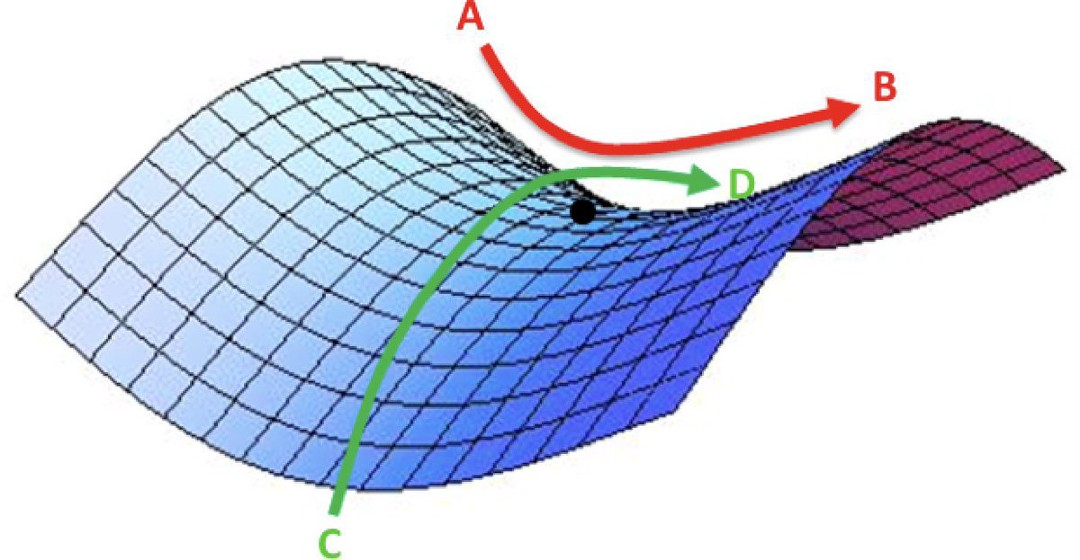
\includegraphics[width=4in]{punkt_siodlowy}
      % \caption[Przykładowy kształt punktu siodłowego - źródło: \url{https://towardsdatascience.com/neural-network-optimization-7ca72d4db3e0}]{Przykładowy kształt punktu siodłowego}
      \caption[Przykładowy kształt punktu siodłowego - źródło: \url{https://towardsdatascience.com}]{Przykładowy kształt punktu siodłowego}
      \label{fig:punkt_siodlowy}
    \end{figure}

    W odpowiedzi na opisane problemy opracowana została technika tak zwanego
    pędu \cite{Momentum}. Ogranicza ona oscylacje spadku gradientu w niewłaściwych kierunkach i
    przyspiesza proces zbiegania rozwiązania. Pęd sprowadza się do dodawania ułamka
    $\gamma$ wektora aktualizacji z poprzedniego kroku algorytmu do bieżącego wektora
    aktualizacji. Przedstawia to poniższy wzór:

    \[V(t)=\gamma \cdot V(t - 1) + \eta \cdot \nabla J(\Theta),\]
    który prowadzi ostatecznie do następującej modyfikacji parametrów:
    \[\Theta = \Theta - V(t).\]

    Nazwa tej metody nawiązuje do pędu znanego z fizyki. Można powiedzieć, że
    w miarę uczenia modyfikacje wag sieci nabierają prędkości we właściwym kierunku, co
    sprawia, że nie są już tak podatne na ewentualne nieprawidłowe zmiany kierunku i
    szybciej osiągają właściwy cel.

    Badacz Yurii Nesterov zauważył jednak zasadniczą wadę związaną z metodą pędu.
    W sytuacji, gdy algorytm przemieszcza się w dół zbocza funkcji celu w żaden
    sposób nie kontroluje, czy znalazł się już na dnie. Gdy je osiąga wartość pędu
    jest dość wysoka, co może spowodować, że punkt optymalny zostanie pominięty
    lub osiągnięty z opóźnieniem. Nesterov zaproponował nieco inne rozwiązanie \cite{Nesterov_momentum}.
    W jego metodzie najpierw wykonywany jest duży skok bazujący na poprzedniej
    wartości pędu, a następnie w nowym, potencjalnym położeniu, obliczana jest wartość 
    gradientu, która dokonuje korekcji miejsca docelowego. Dopiero wówczas dokonywana
    jest rzeczywista aktualizacja parametrów modelu. Metodę tę można przedstawić za
    pomocą następującego wzoru:

    \[V(t)=\gamma \cdot V(t - 1) + \eta \cdot \nabla J(\Theta - \gamma \cdot V(t - 1)),\]
    który prowadzi do aktualizacji:
    \[\Theta = \Theta - V(t).\]

    Argument $\nabla J$, $\Theta - \gamma \cdot V(t - 1)$ odpowiada w tym przypadku za określenie przewidywanego punktu docelowego.
    Pozwala to wyznaczyć wartość gradientu nie dla obecnego położenia modelu na płaszczyźnie
    funkcji celu, ale dla domniemanego położenia osiągniętego w przyszłości. Czyni to
    algorytm optymalizacji bardziej responsywnym na ewentualne zmiany i ogranicza ryzyko
    ominięcia punktu optymalnego ze względu na zbyt dużą wartość pędu.

    Bazując na opisanych tutaj algorytmach przygotowane zostały metody optymalizacji
    dostępne w \textit{TorchFrame}, a zaczerpnięte z biblioteki \textit{PyTorch}. Wiele z nich wprowadza
    również dodatkowe funkcjonalności, z których najistotniejsze opisane zostały w Tabeli \ref{tab:optimizers}.

  \begin{small}
    \begin{longtable}{ |m{3cm}|m{10cm}| }
      \caption{Optymalizatory w \textit{TorchFrame}}
      \label{tab:optimizers}
      \endfirsthead
      \endhead
     \hline
       \textbf{Optymalizator} & \textbf{Opis} \\

     \hline
       \textbf{SGD \cite{SGD}} &

       Algorytm stochastycznego spadku gradientu. Stanowi wariację bazowego spadku
       gradientu polegającą na aktualizowaniu parametrów sieci dla
       każdego przykładu uczącego. Opisuje to następujący wzór:

       \[\Theta = \Theta - \eta \cdot \nabla J(\Theta;x(i);y(i)),\]
       gdzie $\{x(i), y(i)\}$ jest zbiorem poszczególnych par treningowych.

       Stochastyczny spadek gradientu cechuje się częstszymi aktualizacjami i
       zmiennymi oscylacjami na płaszczyźnie funkcji celu. Czyni go to wolniejszym od
       algorytmu bazowego w dążeniu do rozwiązania, jednak zwiększa prawdopodobieństwo odkrycia
       bardziej optymalnych minimów.

       Możliwe jest również zastosowanie opisanych wcześniej mechanizmów pędu oraz
       algorytmu Nesterov'a w celu poprawy wydajności działania tego algorytmu. \\

     \hline
       \textbf{AdaGrad \cite{Adagrad}} &

        Algorytm pozwalający dopasować długość kroku treningowego do poszczególnych
        wag modelu. Parametry rzadko biorące udział w pracy sieci otrzymują wówczas
        większe aktualizacje niż te występujące stosunkowo często. \textit{AdaGrad} nadaje się
        przez to do pracy z rzadkimi zbiorami treningowymi. Wzór prezentujący sposób aktualizacji
        pojedynczego i-tego parametru w sieci prezentuje się następująco:

        \[\Theta_{t+1,i} = \Theta_{t,i} - \frac{\eta}{\sqrt{G_{t,ii} + \epsilon}} \cdot g_{t,i},\]

        gdzie $G_{t,ii}$ jest diagonalną macierzą zawierającą sumy kwadratów gradientów
        wyznaczonych aż do chwili $t$, $g_{t,i}$ jest bieżącą wartością gradientu dla parametru $\Theta_i$, a
        $\epsilon$ oznacza współczynnik wygładzający, zabezpieczający przed ewentualnym dzieleniem
        przez 0.

        Wzór ten oznacza, że \textit{AdaGrad} modyfikuje długość kroku uczącego w każdej iteracji $t$
        dla każdego parametru $i$ bazując na przeszłych wartościach gradientu wyznaczonych
        dla tej wagi.

        Istotną wadą tego optymalizatora jest fakt ciągłego zmniejszania długości
        kroku uczącego ze względu na rosnącą nieustannie wartość sumy kwadratów
        gradientów w mianowniku. W krytycznych przypadkach może to doprowadzić
        do całkowitego zaniku tego kroku, co w konsekwencji prowadzi do
        zablokowania możliwości dalszego treningu sieci. \\

     \hline
       \textbf{AdaDelta \cite{Adadelta}} &

       Algorytm ten stanowi rozszerzenie optymalizatora \textit{AdaGrad}. Rozwiązuje
       trapiący go problem zanikającego kroku treningowego poprzez wprowadzenie
       ograniczenia, co do ilości przeszłych gradientów mających wpływ na aktualizację
       wag w bieżącej iteracji.

       Dodatkowo zamiast przechowywać określoną liczbę przeszłych kwadratów gradientów,
       AdaDelta wyznacza ich sumę poprzez rekursywne definiowanie zanikającej
       średniej wartości przeszłych kwadratów tych gradientów.

       Sposób działania tego mechanizmu opisuje poniższy wzór:

       \[E[g^2]_t = \gamma \cdot E[g^2]_{t-1} + (1 - \gamma) \cdot g^2_t,\]

       gdzie $E[g^2]_t$ oznacza średnią wartość sumy kwadratów gradientów w bieżącej
       iteracji, $E[g^2]_{t-1}$ definiuje tę średnią dla poprzedniego kroku, a
       $g^2_t$ stanowi kwadrat bieżącej wartości gradientu. Parametr $\gamma$
       pełni tutaj podobną rolę, co w przypadku mechanizmu pędu.

       Ostatecznie parametry modelu aktualizowane są zgodnie z następującą formułą:

       \[\Delta \Theta_t = -\frac{\eta}{\sqrt{E[g^2]_t + \epsilon}} \cdot g_t\] \\

     \hline
       \textbf{Adam \cite{Adam}} &

       Optymalizator Adam podobnie jak \textit{AdaDelta} pozwala wyznaczać adaptacyjne długości
       kroku uczącego dla każdego parametru sieci. Przechowuje on również
       eksponencjalnie zanikającą średnią wartość kwadratów przeszłych gradientów $v_t$.
       Poza tym przechowuje również eksponencjalnie zanikającą średnią
       przeszłych gradientów $m_t$ podobną do wartości pędu.

       Wartości $m_t$ oraz $v_t$ są szacunkami odpowiednio pierwszego momentu
       (średnia) oraz drugiego momentu (wariancja niecentrowana), stąd nazwa metody.

       Autorzy Adama zauważyli, że $m_t$ oraz $v_t$, które inicjowane są jako
       wektory zerowe dążą tendencyjnie do zera zwłaszcza podczas początkowych
       iteracji. Aby przeciwdziałać temu procesowi wyznaczane są odpowiednie
       estymaty korekcyjne obu momentów zgodnie ze wzorami:

       \[m'_t = \frac{m_t}{1 - \beta^t_1}\]
       \[v'_t = \frac{v_t}{1 - \beta^t_2}\]

       Na tej podstawie wyznaczana jest reguła aktualizacyjna Adama, postaci:

       \[\Theta_{t+1} = \Theta_t - \frac{\eta}{\sqrt{v'_t} + \epsilon} \cdot m'_t.\]

       Wartości parametrów $\beta_1$, $\beta_2$ oraz $\epsilon$ mogą być dobierane eksperymentalnie,
       jednak rekomendowane jest przyjęcie następujących liczb: $\beta_1 = 0.9$, $\beta_2 = 0.999$, $\epsilon = 10^{-8}$. \\
     \hline
    \end{longtable}
  \end{small}
  
    Wybór odpowiedniego algorytmu optymalizacji nie jest prostym zagadnieniem.
    Ostateczną decyzję powinna poprzedzać matematyczna analiza postawionego
    problemu lub eksperymentalne porównanie dostępnych możliwości. Należy
    pamiętać że czynnik ten ma często kluczowy wpływ na uzyskiwane rezultaty.
    W przypadku prostych zadań optymalizacji najczęściej, choć nie zawsze,
    wystarczające powinny okazać się proste algorytmy takie jak \textit{SGD}.
    Z kolei bardziej złożone problemy z reguły wymagać będą zastosowania metod
    adaptacyjnych takich jak \textit{Adam}, czy \textit{AdaGrad}. Z reguły
    oferują one lepsze rezultaty, jednak za cenę większej złożoności obliczeniowej.
    Wiele zależy również od samego kontekstu użycia. Przykładowo w przypadku
    douczania sieci neuronowej w celu poprawy ostatecznych rezultatów zalecane jest
    użycie algorytmów ze stałą długością kroku treningowego, które w odróżnieniu od
    algorytmów adaptacyjnych mają w takich przypadkach mniejszą tendencję do
    destabilizacji rozwiązania.

    \item \textbf{\textit{Scheduler}} - umożliwia wybór planisty. Odpowiada on za
    modyfikowanie długości kroku treningowego w zależności od aktualnego numeru
    epoki, w jakim znajduje się proces uczenia.

    Jest to istotny element pozwalający dynamicznie dostosowywać krok do
    aktualnego położenia modelu na hiperpłaszczyźnie funkcji celu. Przykładowo
    gdy sieć znajduje się daleko od optimum globalnego, lub gdy wpadnie w jedno z
    optimów lokalnych możliwe jest zwiększenie kroku treningowego, aby przyspieszyć
    proces optymalizacji. Gdy natomiast model znajduje się w pobliżu optimum globalnego
    długość kroku może zostać zmniejszona, co przełoży się na zwiększenie dokładności
    uzyskanych wyników.

    \item \textbf{\textit{Init epoch}} - parametr wskazujący numer epoki od którego
    rozpocznie się trening sieci neuronowej.

    \item \textbf{\textit{Training epochs}} - ilość epok, jaką przejdzie model w danej
    sesji treningowej. W każdej epoce modelowi przekazane zostaną wszystkie dane
    wskazane w zbiorze treningowym.

    \item \textbf{\textit{Training Monitoring Period}} - określa co ile pakietów danych
    obiekt \textit{Trainer} będzie wyświetlał w konsoli dane treningowe, takie jak
    aktualna wartość funkcji kosztu.

    \item \textbf{\textit{Saving Period}} - parametr określający co ile epok
    obiekt \textit{Trainer} będzie dokonywał zapisu pośrednich wyników treningu sieci.

    \item \textbf{\textit{Dataloader Parameters}} - zestaw trzech parametrów.

    \textit{Batch size} określa ilość pojedynczych próbek ze zbioru treningowego które zostaną zgrupowane
    w jeden pakiet danych. W trakcie procesu uczenia sieci wartość funkcji kosztu wyznaczana
    jest dla wszystkich elementów pakietu, a następnie uśredniana i dopiero wtedy
    wykorzystywana przez optymalizator do aktualizacji wag modelu.

    \textit{Shuffle} pozwala określić, czy dane ze zbioru treningowego zostaną
    posortowane, aby uniknąć powtarzalnej kolejności ich przekazywania na wejście
    sieci. Pozwala to lepiej przygotować sieć do pracy z danymi, których nie widziała
    w procesie uczenia.

    \textit{Num workers} to parametr  określający ilość procesów równolegle przetwarzających
    dane i tym samym przyspieszających cały proces treningu.

    \item \textbf{\textit{Retrain}} - wartość \textit{true} tego parametru powoduje, że
    \textit{TorchFrame} podejmie próbę wczytania modelu sieci, optymalizatora oraz
    planisty zgodnie ze ścieżkami zdefiniowanymi w pliku \textit{consts}. Brak którejkolwiek
    ścieżki spowoduje, że dany parametr zostanie zainicjowany losowo, co pozwala
    dotrenować sieć w dowolnej konfiguracji parametrów startowych.

    \item \textbf{\textit{Train on gpu}} - wartość \textit{true} tego parametru sprawi, że
    \textit{TorchFrame} podejmie próbę rozpoznania, czy dostępna jest graficzna jednostka
    obliczeniowa, a następnie przeniesie na nią dane umożliwiając przeprowadzanie
    za jej pomocą obliczeń w celu przyspieszenia procesu uczenia.

    \item \textbf{\textit{Dataset}} - stanowi zbiór parametrów określających sposób
    wstępnego przetwarzania danych w celu przygotowania zbioru uczącego.

    \textit{Name} - zawiera nazwę klasy definiującej sposób przetwarzania
    i przekazywania danych ze zbioru uczącego. Klasa ta powinna być oparta o
    szkielet \textit{BaseDataset} zapewniający sprawny przepływ danych przez framework
    \textit{TorchFrame}.

    \textit{Input conversions} - jest to lista konwersji przeznaczonych do
    przetwarzania danych treningowych przekazywanych na wejście sieci. Każda
    konwersja składa się z nazwy popartej definicją w pliku \textit{conversions} oraz z
    parametrów, których używa w trakcie pracy na danych.

    \textit{Output conversions} - podobnie jak poprzedni parametr jest to lista
    konwersji. Ich implementacja pozwala przygotować zbiór danych wyjściowych
    wykorzystywanych jako punkt odniesienie dla rezultatów pracy sieci przy wyznaczaniu
    wartości funkcji celu.

    \textit{Transforms} - lista transformacji zdefiniowanych w pliku \textit{transforms},
    zapewniających między innymi formatowanie danych do postaci tensorów
    obsługiwanych przez bazowe mechanizmy biblioteki \textit{PyTorch}.

    \item \textbf{\textit{Additional params}} - słownik języka Python, w którym użytkownik
    \textit{TorchFrame} ma możliwość zdefiniowania dowolnych dodatkowych parametrów, jakie
    mogą wydać się pomocne w procesie treningu sieci neuronowej.

    \end{enumerate}

  \subsubsection{Testowanie w \textit{TorchFrame}}
    Podstawą do określenia skuteczności przeprowadzanych treningów sieci neuronowych
    jest nie tylko obserwacja parametrów takich jak wartość funkcji kosztu. Bardzo
    często konieczna jest wizualizacja wyników działania wytrenowanych modeli.
    Komponentowa budowa \textit{TorchFrame} pozwala w łatwy sposób osiągnąć ten cel.
    Na bazie fragmentów wydzielonych z głównej architektury skomponowany został
    system testowy, którego schemat przedstawia Rysunek \ref{fig:torchframetest}.

    Większość przedstawionych na schemacie elementów zachowuje funkcjonalności
    opisane w rozdziale \textit{Architektura TorchFrame}. Istotną różnicą jest
    pojawienie się obiektu \textit{Tester}, którego zadaniem jest przeprowadzanie
    zdefiniowanych przez użytkownika testów. Podobnie jak obiekt \textit{Dataset} bazuje
    on na szkielecie \textit{BaseTester} odpowiadającym za funkcjonalne połączenie z
    resztą frameworka. W ramach tej pracy przygotowane zostały różne warianty
    testowe, jednak elastyczna forma szkieletu pozwala użytkownikom
    na definiowanie własnych scenariuszy.

    Inaczej zachowuje się również \textit{SetupCreator}. Element ten wyposażony został w specjalną
    metodę przeznaczoną do przygotowania środowiska testowego na bazie parametrów
    dostarczonych w pliku konfiguracyjnym JSON.

    Plik ten różni się od tego omawianego w przypadku procesu treningowego. Jego
    zawartość została w znacznym stopniu ograniczona, gdyż proces testowy nie
    wymaga już tak wielu parametrów konfiguracyjnych. Pozwala to zachować
    przejrzystość środowiska testowego i ułatwia rozpropagowanie danych
    w systemie.

    \begin{figure}[h!]
      \centering
      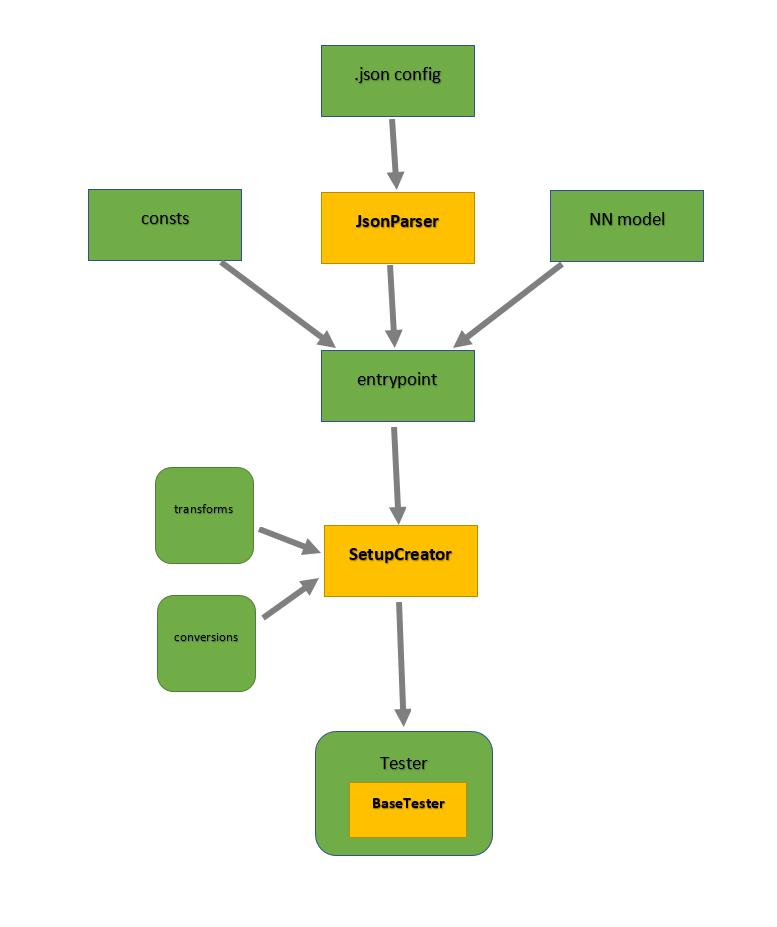
\includegraphics[width=6.5in]{torchframetest}
      \caption[Architektura testowa \textit{TorchFrame} - źródło: Rysunek własny]{Architektura testowa \textit{TorchFrame}}
      \label{fig:torchframetest}
    \end{figure}
